%% This is file `elsarticle-template-1-num.tex',
%%
%% Copyright 2009 Elsevier Ltd
%%
%% This file is part of the 'Elsarticle Bundle'.
%% ---------------------------------------------
%%
%% It may be distributed under the conditions of the LaTeX Project Public
%% License, either version 1.2 of this license or (at your option) any
%% later version.  The latest version of this license is in
%%    http://www.latex-project.org/lppl.txt
%% and version 1.2 or later is part of all distributions of LaTeX
%% version 1999/12/01 or later.
%%
%% The list of all files belonging to the 'Elsarticle Bundle' is
%% given in the file `manifest.txt'.
%%
%% Template article for Elsevier's document class `elsarticle'
%% with numbered style bibliographic references
%%
%% $Id: elsarticle-template-1-num.tex 149 2009-10-08 05:01:15Z rishi $
%% $URL: http://lenova.river-valley.com/svn/elsbst/trunk/elsarticle-template-1-num.tex $
%%
\documentclass[preprint,12pt]{elsarticle}

%% Use the option review to obtain double line spacing
%% \documentclass[preprint,review,12pt]{elsarticle}

%% Use the options 1p,twocolumn; 3p; 3p,twocolumn; 5p; or 5p,twocolumn
%% for a journal layout:
%% \documentclass[final,1p,times]{elsarticle}
%% \documentclass[final,1p,times,twocolumn]{elsarticle}
%% \documentclass[final,3p,times]{elsarticle}
%% \documentclass[final,3p,times,twocolumn]{elsarticle}
%% \documentclass[final,5p,times]{elsarticle}
%% \documentclass[final,5p,times,twocolumn]{elsarticle}

%% if you use PostScript figures in your article
%% use the graphics package for simple commands
%% \usepackage{graphics}
%% or use the graphicx package for more complicated commands
%% \usepackage{graphicx}
%% or use the epsfig package if you prefer to use the old commands
%% \usepackage{epsfig}

%% The amssymb package provides various useful mathematical symbols
\usepackage{graphicx}
\usepackage{amssymb}
\setcounter{tocdepth}{3}
\usepackage{amsmath}
\usepackage{amssymb}
\usepackage{color}
\usepackage{tikz}
\usepackage{pgfplots}
\usepackage{caption}
\usepackage{subcaption}
\usepackage{comment}
\usepackage{booktabs}
\usepackage{nopageno}

\usepackage[algo2e, noend, noline, linesnumbered]{algorithm2e}
%\DontPrintSemicolon

\makeatletter
\newcommand{\pushline}{\Indp}% Indent
\newcommand{\popline}{\Indm}
\makeatother
\DeclareMathOperator{\pess}{pess}
\DeclareMathOperator{\opti}{opti}
\newcommand{\argmax}{\operatornamewithlimits{argmax}}

\captionsetup{compatibility=false}



%\pgfplotsset{compat=newest}
\usetikzlibrary{arrows,shapes,petri}

\newcommand{\bE}{\mathbb{E}}
\newcommand{\cA}{\mathcal{A}}
\newcommand{\cC}{\mathcal{C}}
\newcommand{\cD}{\mathcal{D}}
\newcommand{\cI}{\mathcal{I}}
\newcommand{\cN}{\mathcal{N}}
\newcommand{\cO}{\mathcal{O}}
\newcommand{\cS}{\mathcal{S}}
\newcommand{\cT}{\mathcal{T}}
\newcommand{\cZ}{\mathcal{Z}}
\newcommand{\eg}{{\it e.g.,}~}
\newcommand{\ie}{{\it i.e.,}~}

\definecolor{darkgreen}{RGB}{0,125,0}
\newcounter{mwNoteCounter}
\newcounter{mlNoteCounter}
\newcounter{vlNoteCounter}
\newcounter{bbNoteCounter}
\newcommand{\mwinands}[1]{{\small \color{blue} $\blacksquare$ \refstepcounter{mwNoteCounter}\textsf{[RGG]$_{\arabic{mwNoteCounter}}$:{#1}}}}
\newcommand{\mlanctot}[1]{{\small \color{darkgreen} $\blacksquare$ \refstepcounter{mlNoteCounter}\textsf{[ML]$_{\arabic{mlNoteCounter}}$:{#1}}}}
\newcommand{\vlisy}[1]{{\small \color{red} $\blacktriangle$ \refstepcounter{vlNoteCounter}\textsf{[VL]$_{\arabic{vlNoteCounter}}$:{#1}}}}
\newcommand{\bbosansky}[1]{{\small \color{orange} $\blacktriangle$ \refstepcounter{bbNoteCounter}\textsf{[BB]$_{\arabic{bbNoteCounter}}$:{#1}}}}

\newtheorem{theorem}{Theorem}[section]
\newtheorem{lemma}[theorem]{Lemma}
\newtheorem{proposition}[theorem]{Proposition}
\newtheorem{corollary}[theorem]{Corollary}

\newenvironment{proof}[1][Proof]{\begin{trivlist}
\item[\hskip \labelsep {\bfseries #1}]}{\end{trivlist}}

%% The amsthm package provides extended theorem environments
%% \usepackage{amsthm}

%% The lineno packages adds line numbers. Start line numbering with
%% \begin{linenumbers}, end it with \end{linenumbers}. Or switch it on
%% for the whole article with \linenumbers after \end{frontmatter}.
%% \usepackage{lineno}

%% natbib.sty is loaded by default. However, natbib options can be
%% provided with \biboptions{...} command. Following options are
%% valid:

%%   round  -  round parentheses are used (default)
%%   square -  square brackets are used   [option]
%%   curly  -  curly braces are used      {option}
%%   angle  -  angle brackets are used    <option>
%%   semicolon  -  multiple citations separated by semi-colon
%%   colon  - same as semicolon, an earlier confusion
%%   comma  -  separated by comma
%%   numbers-  selects numerical citations
%%   super  -  numerical citations as superscripts
%%   sort   -  sorts multiple citations according to order in ref. list
%%   sort&compress   -  like sort, but also compresses numerical citations
%%   compress - compresses without sorting
%%
%% \biboptions{comma,round}

% \biboptions{}


\journal{Artificial Intelligence}

\begin{document}

\begin{frontmatter}

%% Title, authors and addresses

%% use the tnoteref command within \title for footnotes;
%% use the tnotetext command for the associated footnote;
%% use the fnref command within \author or \address for footnotes;
%% use the fntext command for the associated footnote;
%% use the corref command within \author for corresponding author footnotes;
%% use the cortext command for the associated footnote;
%% use the ead command for the email address,
%% and the form \ead[url] for the home page:
%%
%% \title{Title\tnoteref{label1}}
%% \tnotetext[label1]{}
%% \author{Name\corref{cor1}\fnref{label2}}
%% \ead{email address}
%% \ead[url]{home page}
%% \fntext[label2]{}
%% \cortext[cor1]{}
%% \address{Address\fnref{label3}}
%% \fntext[label3]{}

\title{Algorithms for Computing Strategies in Two-Player Simultaneous Move Games}

%% use optional labels to link authors explicitly to addresses:
%% \author[label1,label2]{<author name>}
%% \address[label1]{<address>}
%% \address[label2]{<address>}

\author{}

\address{}

\begin{abstract}
Test.
\end{abstract}

\begin{keyword}
%% keywords here, in the form: keyword \sep keyword

%% MSC codes here, in the form: \MSC code \sep code
%% or \MSC[2008] code \sep code (2000 is the default)

\end{keyword}

\end{frontmatter}

%%
%% Start line numbering here if you want
%%
% \linenumbers
%% The Appendices part is started with the command \appendix;
%% appendix sections are then done as normal sections
%% \appendix

%% \section{}
%% \label{}

%% References
%%
%% Following citation commands can be used in the body text:
%% Usage of \cite is as follows:
%%   \cite{key}          ==>>  [#]
%%   \cite[chap. 2]{key} ==>>  [#, chap. 2]
%%   \citet{key}         ==>>  Author [#]

%% References with bibTeX database:

%% main text
\section{Introduction}
\label{sec:intro}

Strategic decision-making in multiagent environments is an imporant problem in artificial intelligence. 
With the growing number of automated agents interacting with humans and with each other, the need to 
understand these strategic interactions at a fundamental level is becoming increasingly important. 
Today, agent interactions occur in many diverse situations, such as e-commerce, social networking, and 
general-purpose robotics, each of which create complex problems that arise from conflicting agent 
preferences. 

Much research has been devoted to developing algorithms that reasoning about or learn multistep 
interactions. For example, adversarial search has been a central topic of artificial intelligence 
since the inception of the field itself, leading to very strong rational behavior in 
Chess~\cite{Campbell02deepblue}. Advances in machine learning for multistep interactions 
(\eg reinforcement learning) have led to self-play algorithms that can achieve master level play 
in Backgammon~\cite{Tesauro95TDGammon}. 

The most common model for these multistage environments is one with strictly {\it sequential} 
iteractions. That is, each player chooses an action when it is their turn to act, and the environment 
generates a new state, with the next player's turn to act, and so on. This model is sufficient in many 
settings, such as Chess and Backgammon, but is not a good representation of the environment when agents 
are allowed to act simultaneously, such as in real-world situations like auctions and autonomous driving. 

In this paper, we present several algorithms for computing strategies in adversarial settings where
players are allowed to act simultaneously. We cover both the offline case, where computation time is 
abundant and strategies are precomputed, and the online case, where computation time is limited and 
agents must search online. We are concerned both with the quality of strategies based on 
their worst-case performance in theory and their obversed performance in practice. We compare and 
contrast the algorithms and choices in the offline and online cases, and thoroughly evaluate each 
algorithm on a suite of games. 

\section{Simultaneous Move Games \label{sec:smg}}

A finite game with simultaneous moves and chance can be described by a tuple 
$(\cN, \cS = \cD\cup\cC\cup\cZ, \cA, \cT, \Delta_c, u_i, s_0)$.
The player set $\cN = \{ 1, 2, c \}$ contains player labels, where 
$c$ denotes the chance player and by convention a player is denoted $i \in \cN$.
$\cS$ is a set of states, with $\cZ$ denoting the terminal states, $\cD$ the states where players make decisions, 
and $\cC$ the possibly empty set of states where chance events occur. $\cA = \cA_1 \times \cA_2$ is the set of 
joint actions of individual players. We denote $\cA_i(s)$ the actions available to player $i$ in state $s \in \cS$. 
The transition function $\cT : \cS \times \cA_1 \times \cA_2 \mapsto \cS$ defines the successor state given a current 
state and actions for both players. $\Delta_c:\cC \mapsto \Delta(\cS)$ describes a probability distribution over 
possible successor states of the chance event. The utility functions 
$u_i : \cZ \mapsto [v_{\min}, v_{\max}] \subseteq \mathbb{R}$ gives the utility of player $i$, with 
$v_{min}$ and $v_{\max}$ denoting the minimum and maximum possible utility respectively. We assume constant-sum 
games: $\forall z \in \cZ, u_1(z) = k - u_2(z)$. 
The game begins in an initial state $s_0$. 
\bbosansky{redefine stochastic successors $\Delta_c:\cS \mapsto \Delta(\cS)$ (identity for non-chance nodes)}
\bbosansky{define value of the matrix games}

\begin{figure}[b!]
\centering
\begin{subfigure}{12cm}
\centering
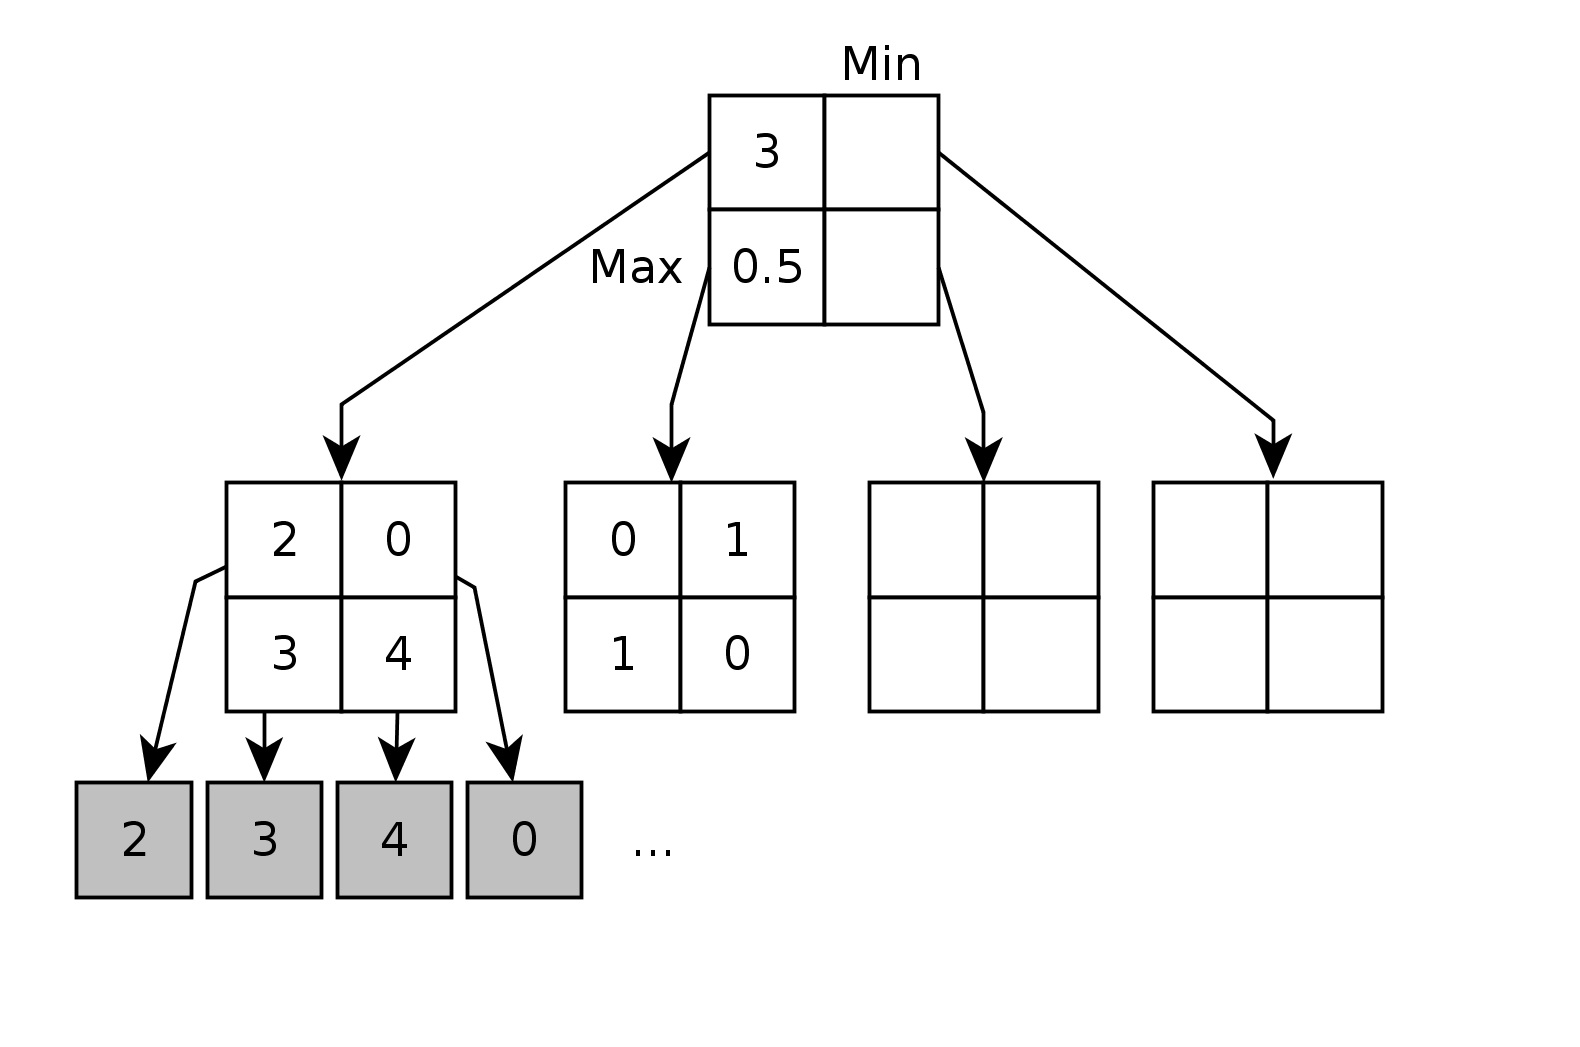
\includegraphics[width=6.0cm]{figures/tree} \hspace{0.03cm} 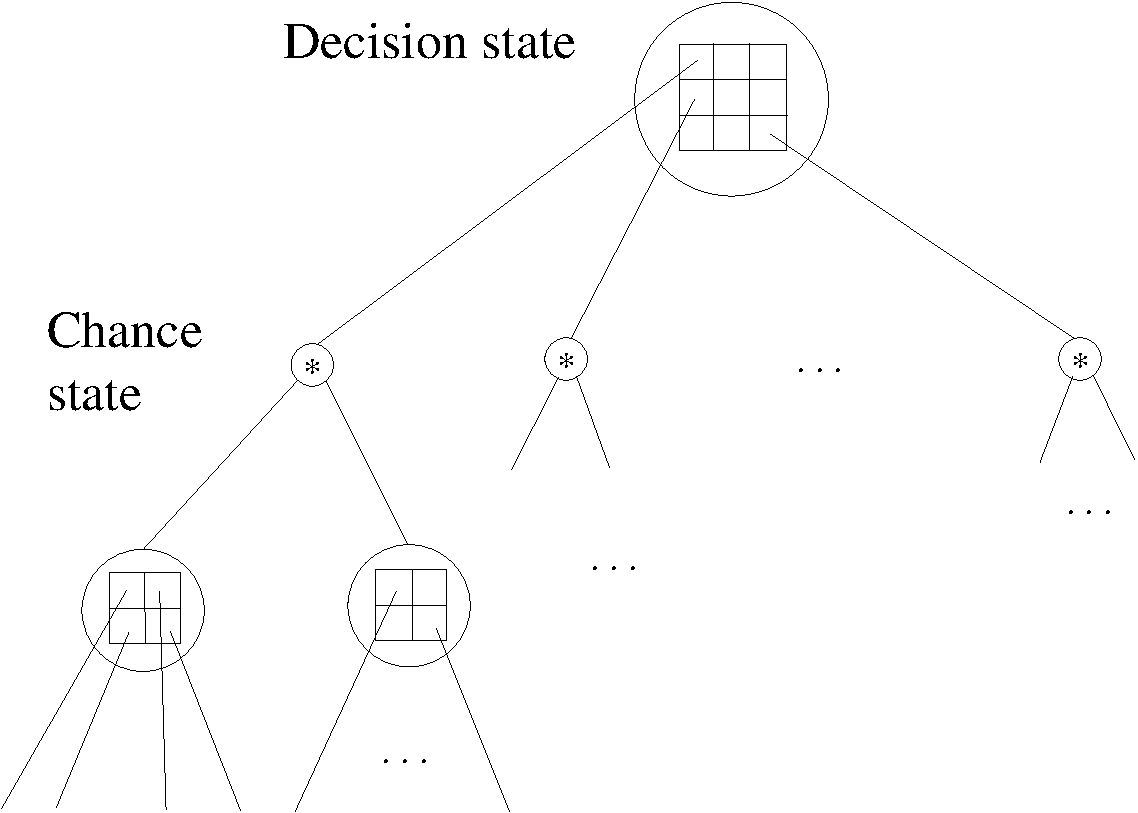
\includegraphics[width=5.5cm]{figures/goof3}\\
\end{subfigure}%\\
\caption{Examples of a two-player simultaneous game without chance nodes (left) which has Matching Pennies as a 
subgame, and a portion of 3-card Goofspiel including chance nodes (right).
The dark squares are terminal states. The values shown are optimal values that could be obtained by backward induction.\\
\label{fig:example}}
\end{figure}

A {\it matrix game} is a single step simultaneous move game with action sets $\cA_1$ and $\cA_2$. 
Each entry in the matrix $A_{rc}$ where $(r,c) \in A_1 \times A_2$ corresponds to a payoff (to player 1) if row $r$ is 
chosen by player 1 and column $c$ by player 2. 
For example, in Matching Pennies, each player has two actions (heads or tails). The row player receives a payoff of 1 
if both players choose the same action and 0 if they do not match. 
Two-player simultaneous move games are sometimes called {\it stacked matrix games} because at every state 
$s$ there is a joint action set $\cA_1(s) \times \cA_2(s)$ that either leads to a terminal state or (possibly after a 
chance transition) to a subgame which is itself another stacked matrix game. 

A {\it behavioral strategy} for player $i$ is a mapping from states $s \in \cS$
to a probability distribution over the actions $\cA_i(s)$, denoted $\sigma_i(s)$. 
Given a profile $\sigma = (\sigma_1, \sigma_2)$, define the probability of reaching a terminal state $z$ under $\sigma$ as 
$\pi^\sigma(z) = \pi_1(z) \pi_2(z) \pi_c(z)$, where each $\pi_i(z)$ is a product of probabilities of the actions taken 
by player $i$ along the path to $z$ ($c$ being chance's probabilities). Define $\Sigma_i$ to be the set of behavioral 
strategies for player $i$. A Nash equilibrium profile in this case is a pair of behavioral strategies optimizing
\begin{equation}\label{eq:ne}
V^* = \max_{\sigma_1 \in \Sigma_1} \min_{\sigma_2 \in \Sigma_2} \bE_{z \sim \sigma}[u_1(z)]
   = \max_{\sigma_1 \in \Sigma_1} \min_{\sigma_2 \in \Sigma_2} \sum_{z \in Z} \pi^\sigma(z) u_1(z).
\end{equation}
In other words, none of the players can improve their utility by deviating unilaterally. 
For example, the Matching Pennies matrix game has a single state and the only equilibrium strategy is to mix equally between 
both actions, \ie play with a {\it mixed strategy} (distribution) of $(0.5, 0.5)$ giving an expected payoff of $V^* = 0.5$. 
If the strategies also optimize Equation \ref{eq:ne} in each subgame starting in an arbitrary state, the equilibrium strategy 
is termed subgame perfect.

In two-player constant sum games a (subgame perfect) Nash equilibrium strategy is often considered to be optimal. It guarantees 
the payoff of at least $V^*$ against any opponent. Any non-equilibrium strategy has its nemesis, which will make it win less 
than $V^*$ in expectation. Moreover, subgame perfect NE strategy can earn more than $V^*$ against weak opponents. After the 
opponent makes a sub-optimal move, the strategy will never allow it to gain the loss back.
The value $V^*$ is known as the minimax-optimal value of the game
and is the same for every equilibrium profile by von Neumann's minimax theorem.

A two-player simultaneous move game is a specific type of two-player imperfect information extensive-form game. 
In imperfect information games, states are grouped into {\it information sets}: two states $s, s' \in I$ if the player 
to act at $I$ cannot distinguish which of these states the game is currently in. Any simultaneous move game can be modeled 
using an information set to represent a half-completed transition, \ie $\cT(s, a_1, ?)$ or $\cT(s, ?, a_2)$. 

The model described above is similar to a two-player finite horizon Markov Game~\cite{Littman94markovgames} with chance 
events. Examples of such games are depicted in Figure~\ref{fig:example}. 

\section{Offline Strategy Computation}


This section focuses on algorithms that compute strategies for simultaneous move games. 
The baseline algorithm for solving simultaneous-move games is backward induction~(Section~\ref{sec:algs:bi}).
Therefore, we start our description of the algorithms focusing on algorithms based on the backward induction, then we introduce algorithms based on no-regret learning and Monte Carlo sampling.
After formally describing the backward induction we present a modification that exploits quick calculation of upper and lower bounds in a simultaneous-move game~(Section~\ref{sec:algs:biab}).
Then, we further improve the algorithm by speeding up the calculation of NE in stage games, exploiting the iterative framework known as the double-oracle algorithm~(Seciton~\ref{sec:algs:doab}).
In Section~\ref{sec:algs:cfros} we present counterfactual regret minimization and its sampling variant outcome sampling. 
Finally, we describe Monte Carlo tree search for simultaneous move games in Section~\ref{sec:algs:smmcts}. 
%\bbosansky{CFR/MCTS introduction}

\subsection{Backward Induction}\label{sec:algs:bi}
Standard backward induction algorithm is based on the depth-first search that in each state of the game evaluates all successors, creates matrix game for the current state, solves the matrix game, and propagates back the value of the matrix game. The pseudocode of the algorithm is depicted in Algorithm~\ref{alg:backwardinduction}. When there is a chance node succeeding the current state $s$, the algorithm directly evaluates all successors of this chance node calculating an expected utility: the value of each subgame rooted in node $s'$ calculated by recursive call is weighted by the probability of the stochastic transition $\Delta_{\cT(s,r,c)}$~(line~\ref{alg:bi:recursive}).

\begin{algorithm2e}[t]
\small
\SetKwInOut{Input}{input}\SetKwInOut{Output}{output}
\Input{$s$ -- current matrix game; $i$ -- searching player}
\If{$s \in \cZ$} {\Return $u_i(s)$} \label{alg:bi:stop1}
\For{$r \in \cA_1(s)$}{
	\For{$c \in \cA_2(s)$} {
	$A_{rc} \leftarrow \sum_{s' \in S \;:\; \Delta_{\cT(s,r,c)}(s') > 0} \Delta_{\cT(s,r,c)}(s')\cdot \textrm{BI}(s',i)$ \label{alg:bi:recursive}\;	
	}
}
$v_s \leftarrow$ solve matrix game $A$\;
\Return $v_s$ \label{alg:bi:stop2}
\caption{Backward Induction.}\label{alg:backwardinduction}
\end{algorithm2e}

Once the algorithm evaluates the value of each possible subgame following the current state $s$, then the matrix game $A$ is complete and the algorithm solves the matrix game $A$ using standard linear program (LP) for solving normal-form games:
\begin{eqnarray}
\max & v_s & \\
\textrm{s.t.} & \sum_{a_i \in \cA_{i}}A_{a_i,a_{-i}} \cdot \delta^{s}_i(a_i) \geq v_s & \forall a_{-i} \in \cA_{-i}\\
& \sum_{a_{i} \in \cA_{i}} \delta^{s}_{i}(a_{i}) = 1 \\
& \delta^{s}_{i}(a_{i}) \geq 0 & \forall a_{i} \in \cA_{i} 
\end{eqnarray}
Using the linear programming, the algorithm computes the value of the matrix game, which is propagated to the predecessor~(line~\ref{alg:bi:stop2}). 
If the algorithm evaluates a terminal state, it directly returns the utility value of the state~(line~\ref{alg:bi:stop1}).

Solving the linear programs is the main computational bottleneck of the backward induction algorithm. Therefore, in the following algorithms, we try to avoid this step of the computation even for the price of multiple traversal of the game tree.

\subsection{Backward Induction with Serialized Alpha-Beta Bounds}\label{sec:algs:biab}
Backward induction algorithm can be easily enhanced by using bounds on the value of sub-games. 
These bounds can be calculated very quickly by using a transformation of a simultaneous-move game into a perfect information extensive-form game.
Consider a matrix game representing a simultaneous choice of both players.
This matrix can be serialized by discarding the notion of information sets; hence, letting one player to play first following by the play of the second player. 
The crucial difference between a serialized and a simultaneous-move matrix game is that the second player to move has an advantage of knowing what action has been played in a serialized game.
Therefore, the value of a serialized game where player $i$ is second to move is an upper bound on the value of the matrix game. 

\begin{figure}
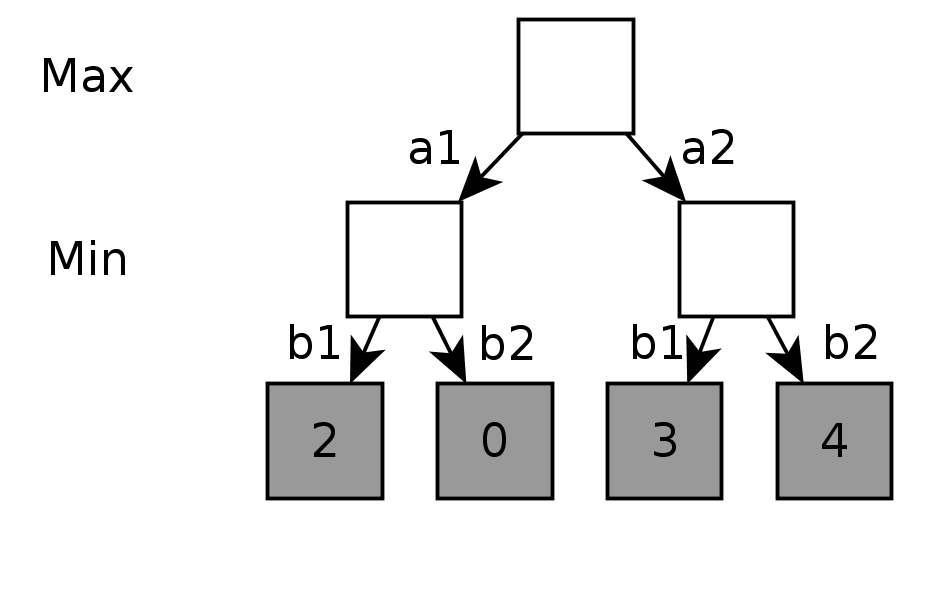
\includegraphics[width=0.45\textwidth]{figures/serialization1-1.png}
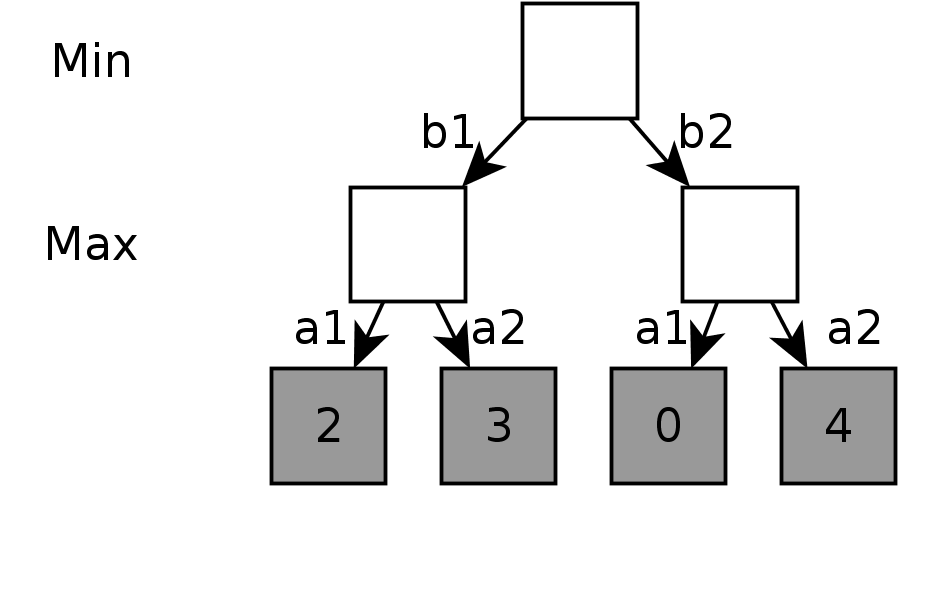
\includegraphics[width=0.45\textwidth]{figures/serialization1-2.png}
\caption{Different serialization of a simultaneous move game.}\label{fig:serialization}
\end{figure}

An example of this serialization is depicted in Figure~\ref{fig:serialization} with the utility value in the leaves depicted only for the first player. 
If this player moves first (the left subfigure), then the value of this serialized game is the lower bound of the value of the game; if this player moves second (the right subfigure), then the value of this serialized game is the upper bound of the value of the game.\vlisy{Write (gray) values into the inner nodes.}
Since the serialized games are zero-sum perfect-information games in the extensive form, they can be solved very quickly by using classical AI algorithm such as alpha-beta or negascout.
If the values of both serialized games are equal, then this is equal also to the value of the game. This situation occurs in our example in Figure~\ref{fig:serialization}, where both serialized games have value equal to $3$.

Obtaining these bounds can speed-up the backward induction algorithm. 
Algorithm~\ref{alg:backwardinduction-ab} depicts the pseudocode.
When the backward induction starts evaluating successors of the current state, the algorithm calculates upper and lower bounds using alpha-beta algorithm on serialized variants of the subgame rooted in the successor $s'$ (lines~\ref{alg:biab:ab1}-\ref{alg:biab:ab2}). The serialized game is solved using standard alpha-beta algorithm, where the second player \vlisy{Unfinished sentence?}
If the bounds are equal, the algorithm stores the value (line~\ref{alg:biab:saving}) instead of performing a recursive call~(line~\ref{alg:biab:recursive}).

\begin{algorithm2e}[t]
\small
\SetKwInOut{Input}{input}\SetKwInOut{Output}{output}
\Input{$s$ -- current matrix game; $i$ -- searching player}
\If{$s \in \cZ$} {\Return $u_i(s)$} \label{alg:biab:stop1}
\For{$r \in \cA_1(s)$}{
	\For{$c \in \cA_2(s)$} {
		$A_{rc} \leftarrow 0$\;
		\For{$s' \in S \;:\; \Delta_{\cT(s,r,c)}(s') > 0$} {
		$v^i_{s'} \leftarrow \textrm{alpha-beta}(s',i)$\; \label{alg:biab:ab1}
		$v^{-i}_{s'} \leftarrow \textrm{alpha-beta}(s',-i)$\; \label{alg:biab:ab2}
		\If{$v^{-i}_{s'} < v^i_{s'}$} {
			$A_{rc} \leftarrow A_{rc} + \Delta_{\cT(s,r,c)}(s')\cdot \textrm{BI}\alpha\beta(s',i)$ \label{alg:biab:recursive}\;	
			}
		\Else{
			$A_{rc} \leftarrow A_{rc} + \Delta_{\cT(s,r,c)}(s')\cdot v^i_{s'}$ \label{alg:biab:saving}
			}
		}
	}
}
$v_s \leftarrow$ solve matrix game $A$\;
\Return $v_s$ \label{alg:biab:stop2}
\caption{Backward Induction with Serialized Bounds}\label{alg:backwardinduction-ab}
\end{algorithm2e}

\subsection{Backward Induction with Double Oracle and Serialized Bounds}\label{sec:algs:doab}
Solving a matrix game can be further improved by using iterative double-oracle algorithm~\cite{McMahan03Planning}. 
First of all, we describe the main principles of the double-oracle algorithm in matrix games, following by describing the application of the algorithm in simultaneous-move game~\cite{Bosansky13Using}.

\subsubsection{Double-oracle Algorithm for Matrix Games}\label{sec:doab}
\begin{figure}
\centering
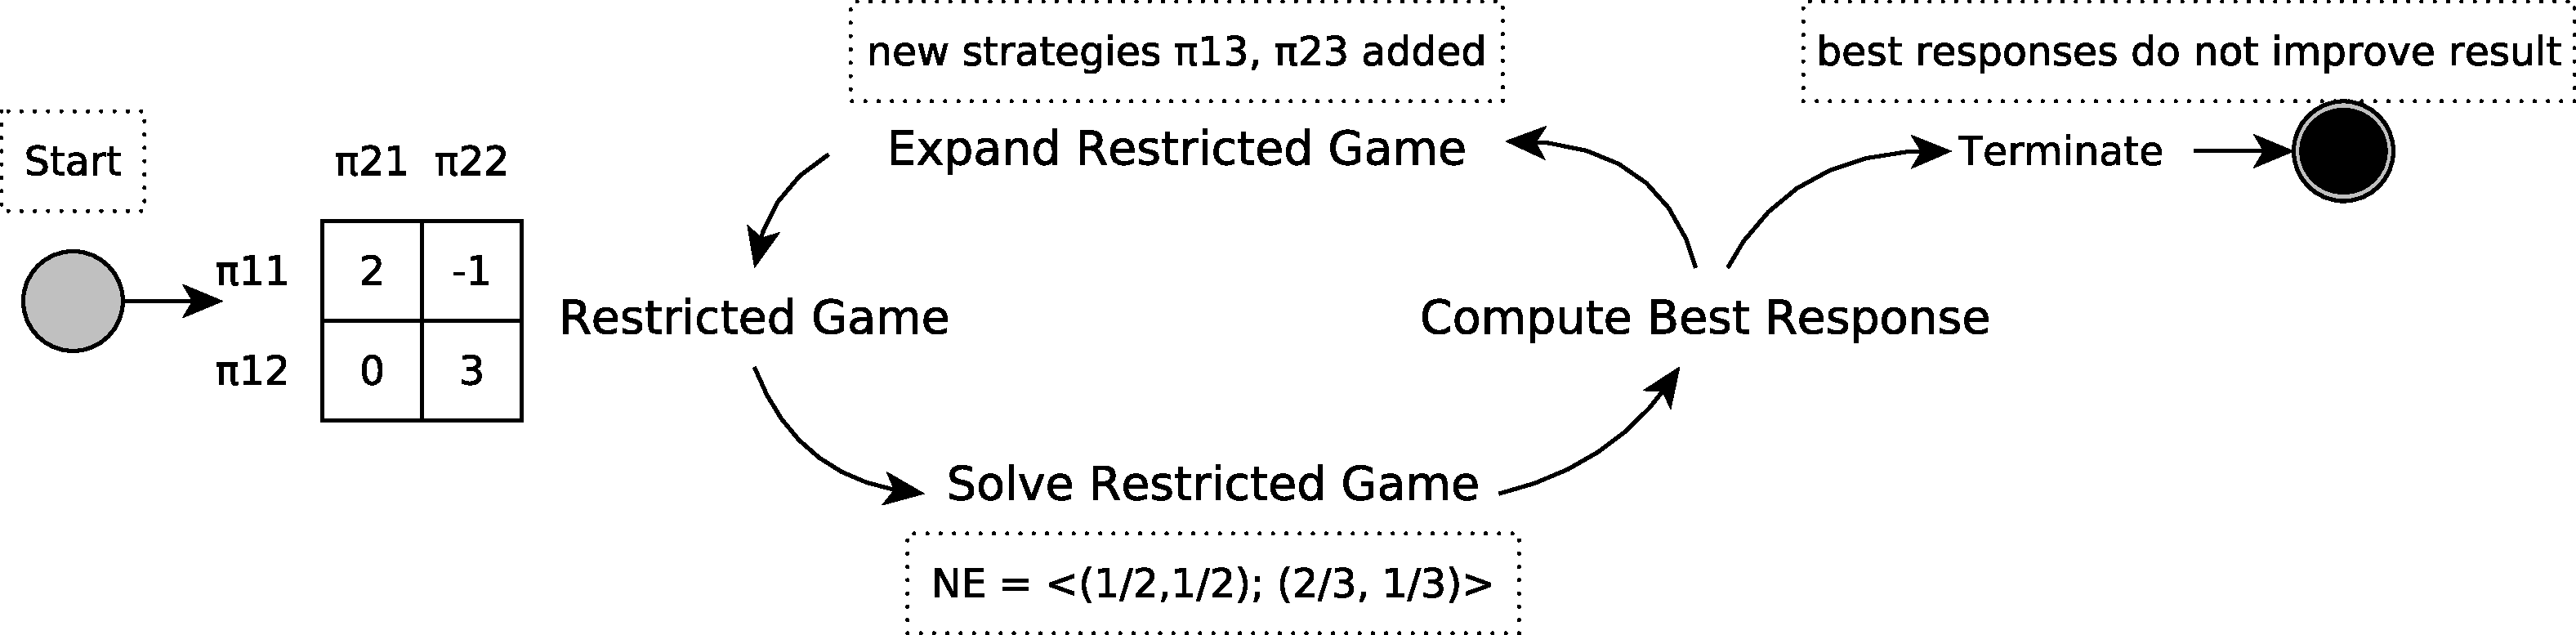
\includegraphics[width=0.8\textwidth]{figures/DO-scheme}
\caption{Schematic of the double-oracle algorithm for a normal-form game.}\label{fig:do-scheme}
\end{figure}

The main goal of the double-oracle algorithm is to find a solution of a matrix game without a need to construct the complete linear program that solves this game. 
The main idea is to create a restricted game by restricting the players to choose only from a limited set of actions.
Then the algorithm iteratively expands the restricted game by allowing the players to choose from new actions.
The new actions are allowed in iterations; each iteration a best response to an optimal strategy of the opponent in the current restricted game is allowed to be played in the restricted game.

Figure~\ref{fig:do-scheme} shows a visualization of the main structure of the algorithm, where the following three steps repeat until convergence:
\begin{enumerate}
\item create a restricted matrix game by limiting the set of actions that each player is allowed to play
\item compute a pair of Nash equilibrium strategies in this restricted game using linear programming
\item for each player, compute a pure best response strategy against the equilibrium strategy of the opponent; pure best response can be \emph{any} action from the original unrestricted game
\end{enumerate}
The best response strategies computed in step 3 are added to the restricted game, the game matrix is expanded by adding new rows and columns, and the algorithm follows with the next iteration. The algorithm terminates if neither of the players can improve the outcome of the game by adding a new strategy to the restricted game; hence, players play best response strategies to the strategy of the opponent. The algorithm maintains the values of expected utilities of the best-response strategies throughout the iterations of the algorithm. These values provide bounds on the value of the original game $v^*$

\subsubsection{Integrating Double-Oracle with Backward Induction}
\begin{algorithm2e}[t]
\small
\SetKwInOut{Input}{input}\SetKwInOut{Output}{output}
\Input{$s$ -- current matrix game; $i$ -- searching player; $\alpha_s,\beta_s$ -- bounds for the game value rooted in state $s$}
\If{$s \in \cZ$} {\Return $u_i(s)$} \label{alg:doab:stop1}
\If{$v_s^{-i} = v_s^i$} {
	\Return $v_s^{i}$
}
initialize $\cA'_i$, $\cA'_{-i}$ with arbitrary actions from $\cA_i, \cA_{-i}$\; \label{alg:doab:init}
\Repeat{$\alpha_s = \beta_s$}{
	\For{$r \in \cA'_i$, $c \in \cA'_{-i}$}{\label{alg:doab:restr1}
		\If{$A'_{rc}$ is not initialized}{
			 $A'_{rc} \leftarrow 0$\;
			\For{$s' \in S \;:\; \Delta_{\cT(s,r,c)}(s') > 0$} {
			$v^i_{s'} \leftarrow \textrm{alpha-beta}(s',i)$\; 
			$v^{-i}_{s'} \leftarrow \textrm{alpha-beta}(s',-i)$\; 
			\If{$v^{-i}_{s'} < v^i_{s'}$} {
				$A'_{rc} \leftarrow A'_{rc} + \Delta_{\cT(s,r,c)}(s')\cdot \textrm{double-oracle}(s',i,v^{-i}_{s'},v^i_{s'})$ \label{alg:doab:recursive}\;	
				}
			\Else{
				$A'_{rc} \leftarrow A'_{rc} + \Delta_{\cT(s,r,c)}(s')\cdot v^i_{s'}$ \label{alg:doab:saving}
				}
			}
		}	
	}
	$\left\langle v_s, \delta' \right\rangle \leftarrow $ solve matrix game $A'$\; \label{alg:doab:NE}
	$\left\langle v^{BR}_i, a^{BR}_{i} \right\rangle \leftarrow $ best-response$(i, \delta'_{-i}, \alpha_s)$\;\label{alg:doab:br1}
	$\left\langle v^{BR}_{-i}, a^{BR}_{-i} \right\rangle \leftarrow $ best-response$(-i, \delta'_{i}, \beta_s)$\; \label{alg:doab:br2}
	$\alpha_s \leftarrow \max(\alpha_s, v^{BR}_i)$,
	$\beta_s \leftarrow \min(\beta_s, v^{BR}_{-i})$\; \label{alg:doab:bounds}
	$\cA'_i \leftarrow \cA'_i \cup \lbrace a^{BR}_i \rbrace$,
	$\cA'_{-i} \leftarrow \cA'_{-i} \cup \lbrace a^{BR}_{-i} \rbrace$ \label{alg:doab:expand}
}
\Return $v_s$ \label{alg:doab:stop2}
\caption{Double Oracle with Serialized Bounds}\label{alg:doab}
\end{algorithm2e}

Double-oracle algorithm for matrix games can be directly incorporated into the backward induction -- instead of immediately evaluating each of the successors of the current game state and solving the linear program, the algorithm can exploit the double-oracle algorithm. Pseudocode in Algorithm~\ref{alg:doab} depicts this integration. In each state of the game, the algorithm initializes the restricted game with an arbitrary action (line~\ref{alg:doab:init}). Afterwards, the algorithm needs to evaluate each of the successors of the restricted game, for which the current value is not known (lines~\ref{alg:doab:restr1}-\ref{alg:doab:saving}). This evaluation is same as for backward induction with alpha-beta algorithm. 

Once all values for the restricted game $A'$ are known, the algorithm solves the restricted game (line~\ref{alg:doab:NE}) and keeps the optimal strategies $\delta'$ of the restricted game. Next, the algorithm calculates best responses for each of the player~(lines~\ref{alg:doab:br1},\ref{alg:doab:br2}), and updates the lower and upper bounds (line~\ref{alg:doab:bounds}). Finally, the algorithm expands the restricted game with best response actions (line~\ref{alg:doab:expand}) until the lower and upper bound are equal. In this case, neither of the best responses improves the current solution from the restricted game; hence, the algorithm has found an equilibrium of the complete unrestricted matrix game corresponding to state $s$.


\begin{algorithm2e}[t]
\small
\SetKwInOut{Input}{input}\SetKwInOut{Output}{output}
\Input{$s$ -- current matrix game; $i$ -- best-response player; $\lambda$ -- bound for the best-response value; $\delta'_{-i}$ -- strategy of the opponent }
$v^{BR}_i \leftarrow \lambda$ \;
$a_i^{BR} \leftarrow \textbf{null}$ \;
\For{$a_i \in \cA_i $\label{alg:br:start}} {%\setminus \cA'_i 
	$v_{a_i} \leftarrow 0$\;
	\For{$a_{-i} \in \cA'_{-i} \;:\; \delta'_{-i}(a_{-i}) > 0$} {\label{alg:br:opp}
		$\lambda_{a_i} \leftarrow \frac{v_i^{BR} - \sum_{a'_{-i} \in \cA'_{-i} \setminus \lbrace a_{-i} \rbrace} \delta'_{-i}(a'_{-i}) \cdot v^i_{\cT(s,a_i,a'_{-i})}}{\delta'_{-i}(a_{-i})}$\; \label{alg:br:bound}
		\If{	$\lambda_{a_i} > v^i_{\cT(s,a_i,a_{-i})}$}{
		continue from line~\ref{alg:br:start} with next $a_i$
		}
		\Else{
		\For{$s' \in S \;:\; \Delta_{\cT(s,a_i,a_{-i})}(s') > 0$} {
%			$v^i_{s'} \leftarrow \textrm{alpha-beta}(s',i)$\; \label{alg:br:ab1}
%			$v^{-i}_{s'} \leftarrow \textrm{alpha-beta}(s',-i)$\; \label{alg:br:ab2}
			\If{$v^{-i}_{s'} < v^i_{s'}$} {
				$v_{a_i,a_{-i}} \leftarrow v_{a_i,a_{-i}} + \Delta_{\cT(s,a_i,a_{-i})}(s')\cdot$ $\textrm{double-oracle}(s',i,v^{-i}_{s'},v^i_{s'})$\label{alg:br:recursive}\;	
				}
			\Else{
				$v_{a_i,a_{-i}} \leftarrow v_{a_i,a_{-i}} + \Delta_{\cT(s,a_i,a_{-i})}(s')\cdot v^i_{s'}$ \label{alg:br:saving}
				}
			}
			$v_{a_i} \leftarrow v_{a_i} + \delta'_{-i}(a_{-i})\cdot v_{a_i,a_{-i}}$\;		
		}
	}
	\If{$v_{a_i} > v_i^{BR}$}{\label{alg:br:max}
		$v_i^{BR} \leftarrow v_{a_i}$\;
		$a_i^{BR} \leftarrow a_i$\label{alg:br:save}
	} 
}
\Return $\langle v_i^{BR}, a_i^{BR} \rangle$ 
\caption{Best Response with Serialized Bounds}\label{alg:br}
\end{algorithm2e}

Next, we describe the algorithm for calculating the best responses. 
The pseudocode of the algorithm is depicted in Algorithm~\ref{alg:br}.
The goal of the algorithm is to find the best action from the original unrestricted game against current strategy of the opponent $\delta'$. 
Throughout the algorithm we use, as before, $v^i_{s'}$ to denote the upper bound of the value of the sub-game rooted in state $s'$ calculated using alpha-beta$(s',i)$. These values are calculated on demand, i.e., they are calculated once needed and cached until the game for state $s$ is not solved.
Moreover, once the algorithm calculates the exact value of a particular subgame, both upper and lower bounds are updated to be equal to actual value of the game. 

The algorithm iteratively tries all actions of player $i$ from the unrestricted game (line~\ref{alg:br:start}). 
Every action $a_i$ is evaluated against the actions of the opponent that are used in the optimal strategy from the restricted game (line~\ref{alg:br:opp}).
Before evaluating against an action of the opponent the algorithm determines, whether the current action of the searching player, $a_i$, can still be the best response action (line~\ref{alg:br:bound}). 
The value $\lambda_{a_i}$ represents the lowest possible expected utility this action must gain against the current action of the opponent $a_{-i}$. 
If this value is strictly higher than the upper bound of the successor (i.e., the value $v^i_{\cT(s,a_i,a_{-i})}$) than the algorithm knows that the action $a_i$ can never be the best response action, and the algorithm proceeds with the next action.
$\lambda_{a_i}$ is calculated by subtracting from the current best response value ($v_i^{BR}$) upper bound of the expected value against all other actions of the opponent ($v^i_{\cT(s,a_i,a'_{-i})}$). Recall, that these values are updated once the algorithm calculates exact values.

If the currently evaluated action $a_i$ can still be the best response, the value of the successor is determined (first by comparing the bounds). Once the expected outcome against all actions of the opponent is evaluated, the expected value of action $a_i$ is compared against the current best-response value (line~\ref{alg:br:max}) and saved, if the expected utility is higher~(line~\ref{alg:br:save}).

\subsection{Simultaneous-Move Monte Carlo Tree Search (SM-MCTS)} \label{sec:algs:smmcts}

Monte Carlo Tree Search (MCTS) is a simulation-based state space search algorithm often used
in game trees. The nodes in the tree represent game states. The main idea is to iteratively run
simulations to a terminal state, incrementally growing a tree rooted at the initial state of the game. In
its simplest form, the tree is initially empty and a single leaf is added each iteration. Each iteration
starts by visiting nodes in the tree, selecting which actions to take based on a selection function and
information maintained in the node. Consequently, the algorithm transitions to a successor state. When a
node is visited whose immediate children are not all in the tree, the node is expanded by adding a
new leaf to the tree. Then, \emph{a rollout policy} (e.g., random action selection) is applied from the new
leaf to a terminal state. The outcome of the simulation is then returned as a reward to the new leaf
and the information stored in the tree is updated.

\begin{algorithm2e}[t]
\small
\SetKwInOut{Input}{input}\SetKwInOut{Output}{output}
\Input{$s$ -- current state of the game}
\If{$s \in \cZ$} {
	\Return $u_1(s)$\;
}
\If{$s \in \cC$} {
        Sample $s' \sim \Delta_c(s)$\;
	\Return SM-MCTS($s'$)\;
}
\If{$s \in T$} {
	$(a_1, a_2) \leftarrow$ \emph{\underline{Select}}$(s)$\;\label{alg:smmcts:select}
	$s' \leftarrow \cT(s,a_1,a_2)$\;
	$v_{s'} \leftarrow $ SM-MCTS($s'$)\;\label{alg:smmcts:reccall}
	\emph{\underline{Update}}$(s,a_1,a_2,v_{s'})$\;\label{alg:smmcts:up}
	\Return $v_{s'}$\;
}
\Else{
	$T \leftarrow T \cup \lbrace s \rbrace$\;
	$v_{s} \leftarrow$ Rollout($s$)\;
	\Return $v_{s}$\;
}
\caption{Simultaneous Move Monte Carlo Tree Search}\label{alg:smmcts}
\end{algorithm2e}

We first present a generic template of MCTS algorithms for simultaneous move games (SM-MCTS) and then explain specific algorithms derived form this template.
Algorithm~\ref{alg:smmcts} describes a single iteration of the SM-MCTS. 
$T$ represents the MCTS tree, in which each state is represented by one node.
Every node $s$ maintains algorithm-specific statistics about the iterations that previously used this node.
The template can be instanciated by specific implementations of the updates of the statistics on line~\ref{alg:smmcts:up} and the selection based on these statistics on line \ref{alg:smmcts:select}.
In the terminal states, the algorithm returns the value of the state for the first player (line 2).
In the chance nodes, the algorithm selects one of the possible next stated based on the chance distribution (line 4).
If the current state has a node in the current MCTS tree $T$, the statistics in the node are used to select an action for each player (line~\ref{alg:smmcts:select}.
These actions are executed (line 8) and the algorithm is called recursively on the resulting state (line 9).
The result of this call is used to update the statistics maintained for state $s$ (line~\ref{alg:smmcts:up}).
If the current state is not stored in tree $T$, it is added to the tree (line 13) and its value is estimated usinf the rollout policy (line 14).

Different algorithms can be the bases for the selection functions (e.g., UCB~\cite{UCB}, Exp3~\cite{Auer2003Exp3}).
We now present the variants of SM-MCTS that were consistently the most successful in previous works, though more variants can be found in~\cite{Perick12Comparison,Lanctot13Tron,Tak14smmcts}.
Several examples are depicted in \cite{Tak14smmcts}. 

\subsubsection{Decoupled Upper-confidence Bound applied to Trees}\label{sec:duct}

The most common selection function for SM-MCTS is the Decoupled Upper-confidence Bound applied to Trees(DUCT).
For selection and updates, it executes the well-known UCT \cite{UCT} algorithm independently for each of the players in each nodes.
The statistics stored in search nodes are independently computed for each action of each player. For player $i\in \cN$ and action $a_i \in \cA_i(s)$ the reward sums $X_{a_i}$ and the number of times the action was used $n_{a_i}$ are maintained.
When a joint action needs to be selected by the \emph{\underline{Select}} function, an action that maximizes the UCB value over their reward estimates is selected for each player independently:
\begin{equation}
a_i = \argmax_{a_i \in \cA_i(s)}{ \left\{ \bar{X}_{a_i} + C_i \sqrt{\frac{\log n_s}{n_{a_i}}} \right\} },
  \mbox{ where } \bar{X}_{a_i} = \frac{X_{a_i}}{n_{a_i}} \mbox{ and } n_s=\sum_{b_i \in \cA_i(s)} n_{b_i}.
\end{equation}
\noindent The \emph{\underline{Update}} function increases the visit count and rewards for each player $i$ and its selected action $a_i$ using $X_{a_i} \leftarrow X_{a_i} + u_i$
and $n_{a_i} \leftarrow n_{a_i} + 1$.



Note that UCT does not define what happens which action is selected if multiple actions have identical value in the maximization. It is not relevant in sequential games, but it can have large impact in simultaneous move games. Consider the following matrix game
\begin{tiny}
$\left(\begin{array}{cc}
0 & 1\\
-1 & 0
\end{array}\right)$
\end{tiny}.
It has only one NE, such that both players play the first action. However, DUC selecting the first or the last action among the options with the same value will always get only the rewards 0 and the bias term will cause the players to round-robin over the diagonal indefinitely. This is clearly not optimal, as each player can than improve by playing first action with probability 1. However, if we choose the action to play randomly among the once with the same probability, DUCT will quickly converge to the optimal solution. Therefore, we use the randomized variant in our implementation.

After all the simulations are done, there are two options how to determine the resulting action to play.
The more standard option is to choose for each state the action $a_i$ that maximizes $n_{a_i}$ for each player $i$.
This is suitable mainly for games, in which using mixed strategy is not necessary.
Alternatively, the action to play in each state can be determined based on the mixed strategy obtained by normalizing the visit counts of each action 
\begin{equation}
\sigma_i(a_i) = \frac{n_{a_i}}{\sum_{b_i\in \cA_i(s)} n_{b_i}}.
\end{equation}
We call the former DUCT(max) and the latter DUCT(mix).
Using the first method will certainly not make the algorithm converge to a Nash equilibirum, because the game may require a mixed strategy.
The second has been shown not to converge to a Nash equilibrium as well; a counter-example in Rock, Paper, Scissors with biased payoffs is shown in \cite{Shafiei09}.

Even though DUCT is not guaranteed to converge to the optimal solution, it is often very successful in practice.
It has been used in and general game playing~\cite{Finnsson12}, in the Internet card game Urban Rivals~\cite{Teytaud11Upper},
and in the simultaneous move game Tron~\cite{Perick12Comparison}.
\mlanctot{Is there an earlier Tron paper where it was used?}
Note that DUCT is different than UCT run on a game that is transformed to perfect information by serialization of the simultaneous moves,
because in the latter case one player has the advantage of knowing what the other player chose at every stage.
\vlisy{Possibly mention convergence in games with pure strategies.}

\subsubsection{Exponential-weight algorithm for Exploration and Exploitation}\label{sec:exp3}

The second most common instantiation of SM-MCTS is to use the Exponential-weight algorithm for Exploration and Exploitation (Exp3) algorithm \cite{Auer2003Exp3} independently for each of the players.
In Exp3, each player maintains an estimate of the sum of rewards for each action, denoted $\hat{X}_{a_i}$. The joint action produced by \emph{\underline{Select}} is composed of an action independently selected for each player.
The probability of using action $a_i$ is proportional to the exponential of the reward estimates:
\begin{equation}\label{eq:exp3select}
\sigma_i(a_i) = \frac{(1-\gamma) \exp(\eta \hat{X}_{a_i})}{\sum_{b_i \in \cA_i(s)} \exp(\eta \hat{X}_{b_i})} + \frac{\gamma}{|\cA_i(s)|},
  \mbox{ where } \eta = \frac{\gamma}{|\cA_i(s)|}.
\end{equation}

This standard formulation of Exp3 is suitable for deriving its properties, but a straightforward implementation of this formula leads to problems with numerical stability. Both the numerator and denominator of the fraction can quickly become too large. For this reason, numerically more stable formulations has been suggested, e.g., in \cite{Lanctot13Goofspiel} and \cite{Cowling12ISMCTS}. We use the following quivalent formulation from \cite{Cowling12ISMCTS}:
\begin{equation}
\sigma^t_i(a_i) = \frac{(1-\gamma)}{\sum_{b_i \in A_i(s)}\exp(\eta(\hat{X}_{b_i}-\hat{X}_{a_i}))}
\end{equation}

The update after selecting actions $(a_1,a_2)$ and obtaining a simulation result $v_1$ normalizes the result to the unit interval for each player by
\begin{equation}
u_1 \leftarrow \frac{(v_1 - v_{min})}{v_{max} - v_{min}};\;\; u_2 \leftarrow (1-u_1)
\end{equation}
and adds to the corresponding reward sum estimates the reward divided by the probability that the action was played by the player using
\begin{equation}
\hat{X}_{a_i} \leftarrow \hat{X}_{a_i} + \frac{u_i}{\sigma_i(a_i)}.
\end{equation}
Dividing the value by the probability of selecting the corresponding action makes $\hat{X}_{a_i}$ estimate the sum of rewards over all
iterations, not only the once where $a_i$ was selected.

As the final strategy, after all iterations are executed, the algorithm computes the \emph{average strategy} of the Exp3 algorithm over all iterations for each player. After $n$ iterations in the particular node, it is
\begin{equation}
\bar{\sigma}^t_i(a_i) = \frac{1}{n}\sum_{t=1}^n \sigma^t_i(a_i).
\end{equation}
In our implementation, we maintain the cumulative sum and normalize it to obtain the average strategy after the iterations.

Previous work \cite{Teytaud11Upper} suggests first removing the samples caused by the exploration.
This modification proved to be useful also in our experiments and it has been shown not to reduce the performance substantially in the worst case \cite{kovarik}, \mlanctot{Add missing reference} so as the resulting final mixed strategy, we use
\begin{equation}
\bar{\sigma}_i(a_i) \leftarrow \max\left(0, \bar{\sigma}_i(a_i) - \frac{\gamma}{|\cA_i(s)|}\right),
\end{equation}
normalized to sum to one.

\subsubsection{Regret Matching} \label{sec:rm}

This variant applies regret matching \cite{Hart00} to the current estimated matrix game at each stage. The statistics stored by this algorithm in each node are the use count of each joint action ($n_{a_1a_2}$), the sum of rewards for each joint action ($X_{a_1a_2}$). Furthermore, the algorithm for each player $i$ maintains a cumulative regret $r^i_{a_i}$ for having played $\sigma_i^t$ instead of $a_i \in \cA_i(s)$ on iteration $t$, initially set to 0. The regret values $r^i_{a_i}$ are maintained separately by each player, as in DUCT. However, the updates uses a value that is a function of the joint action space. 

On iteration $t$, function \emph{\underline{Select}} first builds
each player's current strategies from the cumulative regrets. Define $x^+ = \max(x,0)$,
\begin{equation}
\label{eq:rm}
\sigma^t_i(a_i) = \frac{r^{i+}_{a_i}}{R^+_{sum}} \mbox{ if } R^+_{sum} > 0 
\mbox{ oth. } \frac{1}{|\cA_i(s)|}, \mbox{ where } R^+_{sum} = \sum_{b_i \in \cA_i(s)}{r^{i+}_{b_i}}.
\end{equation}
The main idea is to adjust the strategy by assigning higher weight proportionally to actions based on the regret of having not taken them over the long-term.
To ensure exploration, an $\gamma$-on-policy sampling procedure similar to Equation~\ref{eq:exp3select} is used
choosing action $a_i$ with probability $\gamma/|\cA(s)| + (1-\gamma) \sigma^t_i(a_i)$.

\emph{\underline{Update}} adds regret accumulated at the iteration to
the regret tables $r^i$. Suppose joint action $(a_1,a_2)$ is
sampled from the selection policy and utility $v_1$ is returned from the recursive call on line~\ref{alg:smmcts:reccall}.
Label $reward(b_1,b_2) = \frac{X_{b_1b_2}}{n_{b_1b_2}}$ if
$(b_1,b_2) \not= (a_1,a_2)$, or $v_1$ otherwise. The updates to the regret are:
\begin{eqnarray}
\forall b_1 \in \cA_1(s), ~~  r^1_{b_1} \leftarrow r^1_{b_1} + ( reward(b_1, a_2) - v_1 ),\\
\forall b_2 \in \cA_2(s), ~~  r^2_{b_2} \leftarrow r^2_{b_2} - ( reward(a_1, b_2) - v_1).
\end{eqnarray}
%\noindent and average strategy updates for each player, $\bar{\sigma}^i_s[a] \leftarrow \bar{\sigma}^i_s[a] + \sigma^t_i(s,a).$

After all simulations, the strategy to play in state $s$ is defined by the mean strategy used in the corresponding node as in case of Exp3.

\subsection{Counterfactual Regret Minimization and Outcome Sampling} \label{sec:algs:cfros}

Counterfactual Regret (CFR) is a notion of regret at the information set level for extensive-form games with imperfect information~\cite{CFR}.
The CFR algorithm iteratively learns strategies in self-play, producing approximate equilibrium strategues over time. 

Define a {\it history} as a sequence of actions taken by all players (including chance) that starts from the beginning of the game. 
A history $h'$ is a prefix of another history $h$, denoted $h' \sqsubset h$, if $h$ contains $h'$ (as a prefix sequence of actions).  
The {\it counterfactual value} of reaching information set $I$ is the expected payoff given that player $i$ played to reach $I$, the opponents played
$\sigma_{-i}$ and both players played $\sigma$ after $I$ was reached:
\begin{equation}
\label{eq:cfv}
v_i(I,\sigma) = \sum_{(h,z) \in Z_I} \pi^{\sigma}_{-i}(h) \pi^{\sigma}_{i}(h,z) u_i(z), 
\end{equation}
where $Z_I = \{ (h,z)~|~z \in Z, h \in I, h \sqsubset z \}$.
Suppose, at time $t$, player $i$ plays with strategy $\sigma^t_i$.
Define $\sigma^t_{I \rightarrow a}$ as identical to $\sigma^t$ except at $I$ action $a$ is taken with probability $1$.
The counterfactual regret of not taking $a \in A(I)$ at time $t$ is $r^t(I,a) = v_i(I,\sigma^t_{I \rightarrow a}) - v_i(I,\sigma^t)$.
The CFR algorithm maintains the cumulative regret $R^T(I,a) = \sum_{t=1}^T r^t(I,a)$, for every action at every information set.
Then, the distribution at each information set for the next iteration $\sigma^{T+1}(I)$ is obtained individually using
regret-matching~\cite{Hart00}. The distribution is proportional to the positive portion of the individual actions' regret:
\begin{equation*}
\label{eq:rm}
\sigma^{T+1}(I,a) = \left\{
\begin{array}{ll}
R^{T,+}(I,a) / R^{T,+}_{sum}(I) & \mbox{if } R^{T,+}_{sum}(I) > 0 \\ 
1 / |A(I)|                   & \mbox{otherwise,}
\end{array} \right.
\end{equation*}
where $x^+ = \max(0,x)$ for any term $x$, and $R^{T,+}_{sum}(I) = \sum_{a' \in A(I)} R^{T,+}(I,a')$. 
Furthermore, the algorithm maintains for each information set the average   strategy profile
\begin{equation}
%\bar{\sigma}^T(I,a) = \frac{1}{T}\sum_{t=1}^T \sigma^t(I,a).
\bar{\sigma}^T(I,a) = \frac{\sum_{t=1}^T \pi^{\sigma^t}_i(I) \sigma^t(I,a)}{\sum_{t=1} \pi^{\sigma^t}_i(I)}, 
\end{equation}
where $\pi^{\sigma^t}_i(I) = \sum_{h \in I}\pi^{\sigma^t}_i(h)$.
The combination of the counterfactual regret minimizers in individual information sets also minimizes the overall 
average regret \cite{CFR}, and hence the average profile is a  $2\epsilon$-equilibrium, with $\epsilon \rightarrow 0$
as $T \rightarrow \infty$.

Monte Carlo Counterfactual Regret Minimization (MCCFR) applies CFR to sampled portions of the games~\cite{Lanctot09Sampling}.
In the {\it outcome sampling} (OS) variant, a single terminal history $z\in Z$ is sampled in each iteration.
The algorithm updates the regret in the information sets visited along $z$ using the
{\it sampled counterfactual value},
\begin{equation}
\tilde{v}_i(I,\sigma) = \left\{
\begin{array}{ll}
\frac{1}{q(z)} \pi^{\sigma}_{-i}(z) \pi^{\sigma}_{i}(h,z) u_i(z) & \mbox{if } (h,z) \in Z_I\\
0  & \mbox{otherwise,}
\end{array} \right.
\label{eq:scv}
\end{equation}
where $q(z)$ is the probability of sampling $z$.
As long as every $z \in Z$ has non-zero probability of being sampled, $\tilde{v}_i(I,\sigma)$ is an unbiased estimate of $v(I,\sigma)$
due to the importance sampling correction ($1/q(z)$). For this reason, applying CFR updates using these sampled counterfactual regrets
$\tilde{r}^t(I,a) = \tilde{v}_i(I,\sigma^t_{I \rightarrow a}) - \tilde{v}_i(I,\sigma^t)$
on the sampled information sets values also eventually converges to the approximate equilibrium of the game with high probability.
The required number of iterations for convergence is much larger, but each iteration is much faster.

%Pseudocode of outcome sampling is presented in the next subsection.

% Will put pseudocode in the Online part..?
%\begin{algorithm2e}[t]
%\small
%\SetKwInOut{Input}{input}\SetKwInOut{Output}{output}
%\Input{game $g$}
%\Return 1
%\caption{Outcome Sampling MCCFR}\label{alg:os}
%\end{algorithm2e}

\subsubsection{Online Outcome Sampling} \label{sec:oos}

Online Outcome Sampling (OOS) is a version of outcome sampling MCCFR described in 
Section~\ref{sec:algs:cfros}. It resembles MCTS in that it builds its tree incrementally, however it 
is based on outcome sampling MCCFR rather than on UCB. The algorithm as applied to full imperfect information
games is found in~\cite{Lanctot14OOS}. Here, we describe a simplified version specifically designed for 
simultaneous move games. 

% Note, mlanctot: \ElsIf breaks compilation for me but \ElseIf works
%bb: Interestingly, \ElseIf does not work for me, but \ElsIf does ... maybe different versions of algorithm2e ?
\begin{algorithm2e}[t]
\small
\SetKwInOut{Input}{input}\SetKwInOut{Output}{output}
\Input{$h$ -- current state of the game; $i$ -- current player; $\pi_i$ -- reach probability for player $i$; $\pi_{-i}$ -- reach probability for opponent of $i$, $s$ -- sample reach probability}
  \lIf{$h \in Z$}{\Return $(s, u_i(z))$} \label{alg:terminal}
  \ElsIf{$h$ is a chance node}{
    Sample outcome $a$ with probability $\Pr(a)$ \;
    \Return OOS$(ha, i, \pi_i, \pi_{-i}, s \cdot \Pr(a))$\;
  }
  $I \gets $ information set of player $P(h)$ at $h$ \;
  Sample $a \sim \Phi(I, i, \epsilon)$ with prob. $\Pr(a)$ \; \label{alg:sample}
  \If{$I$ is not in memory}{
    Add $I$ to memory \;
    $\sigma(I) \leftarrow \mbox{Unif}(A(I))$ \;
    $(q(z), u_i(z)) \gets $ Playout$(ha, s \cdot \Pr(a))$ \;         \label{alg:playout}
  }
  \Else{
    $\sigma(I) \gets $ RegretMatching$(R_I)$ \;
    $\pi_{P(h)}' \gets \sigma(I,a)\pi_{P(h)}$ \;    \label{alg:newreaches1}
    $\pi_{-P(h)}' \gets \pi_{-P(h)}$ \;             \label{alg:newreaches2}
    $(q(z), u_i(z)) \gets$ OOS$(ha, i, \pi_i', \pi_{-i}', s \cdot \Pr(a))$ \;
  }
  \For{$a' \in A(I)$}{
    \If{$P(h) = i$}{
      Update $R_I[a']$ for each $a' \in A(I)$ using $\tilde{r}^t(I,a)$ according to Eq.~\ref{eq:scv}
    }
    \Else{
      Update $S_I[a'] \gets S_I[a'] + \frac{1}{s} \pi_{-i} \sigma(I,a')$ for each $a' \in A(I)$ \;  \label{alg:avgstrat}
    }
  }
  \Return $(q(z), u_i(z))$ \;   \label{alg:returnend}
  \vspace{0.1cm}
  \caption{Simultaneous Move Online Outcome Sampling. \label{alg:oos}}
\end{algorithm2e}



One iteration of the algorithm requires, as input, the current state of the game and a player role $i$. 
Each iteration the player role $i$ is alternated. As the algorithm is applied to the imperfect information 
representation of the simultaneous move game (described in Section~\ref{sec:smg}), we use histories $h$ 
and information sets $I$ rather than states. 

An information set tree is incrementally built, starting with the searching player's root information set.
An information set stores two tables: $R_I$ stores the cumulative regret $R^T(I,a)$ for each action, 
and average strategy table $S_I$ which stores the cumulative average strategy contribution for each action. 
An $\epsilon$-on-policy sampling distribution used to sample actions, defined as
\begin{equation*}
\label{eq:ossample}
\Phi(I,i,\epsilon) = \left\{
\begin{array}{ll}
\epsilon \cdot \mbox{Unif}(A(I)) + (1-\epsilon)\sigma_i(I) & \mbox{if } P(I) = i\\ 
\sigma_i(I)                                          & \mbox{otherwise,}
\end{array} \right.
\end{equation*}
and denote $\Phi(I,i,\epsilon,a)$ the probability of sampling $a \in A(I)$.







\section{Online Search}

\subsection{Iterative Deepening Backward Induction Algorithms}

\subsection{Online Outcome Sampling}

\section{Empirical Evaluation}

\section{Conclusion}


\bibliographystyle{model1-num-names}
\bibliography{sm-journal}

%% Authors are advised to submit their bibtex database files. They are
%% requested to list a bibtex style file in the manuscript if they do
%% not want to use model1-num-names.bst.

%% References without bibTeX database:

% \begin{thebibliography}{00}

%% \bibitem must have the following form:
%%   \bibitem{key}...
%%

% \bibitem{}

% \end{thebibliography}


\end{document}

%%
%% End of file `elsarticle-template-1-num.tex'.
